%#########################################################################
\chapter{Oscilaciones}
\label{cha:oscillations}

El concepto de oscilación es ampliamente usado en ciencia y se aplica para
cualquier cantidad que presente fluctuaciones o perturbaciones en función 
del tiempo, ya sean periódicas o no. En este capítulo se presentan algunos
ejemplos de oscilaciones para sistemas mecánicos y electromagnéticos, que 
a pesar de su simplicidad, permiten ahondar en los detalles físicos de este
tipo de fenómenos.

\

La forma estándar de abordar un problema en una disciplina científica 
consiste en el estudio de situaciones ideales y muy particulares para llegar 
luego, usando refinamientos y consideraciones posteriores, a descripciones 
realistas y más generales. Por este motivo se comienza con demostraciones 
computacionales aplicadas a sistemas ideales, como el péndulo simple, el 
sistema masa resorte, etc. En demostraciones siguientes se abordarán 
aspectos cada vez más complejos de estos sistemas.
%#########################################################################


\
%*************************************************************************
\section{Demostración 1: Péndulo Simple Ideal}
\label{sec:DEMO2_01}
\rule{14cm}{0.5mm}

Como primer caso se aborda el péndulo simple. Este consiste en un sistema
de una masa $m$ con dimensión despreciable y bajo la acción de la 
gravedad $\bds g$, además pende de una cuerda tensa de longitud $l$ y sujeta
en un punto fijo. A partir de la figura \ref{fig:simple_pendulum}, la 
ecuación de movimiento está dada por


%.........................................................................
%Movement equation
\eq{eq:simple_pendulum}
{m\dtot{^2\bds r}{t^2} = m\bds g + \bds T}
%.........................................................................

\newpage
%.........................................................................
%Simple Pendulum
\begin{figure}[htbp]
	\centering
	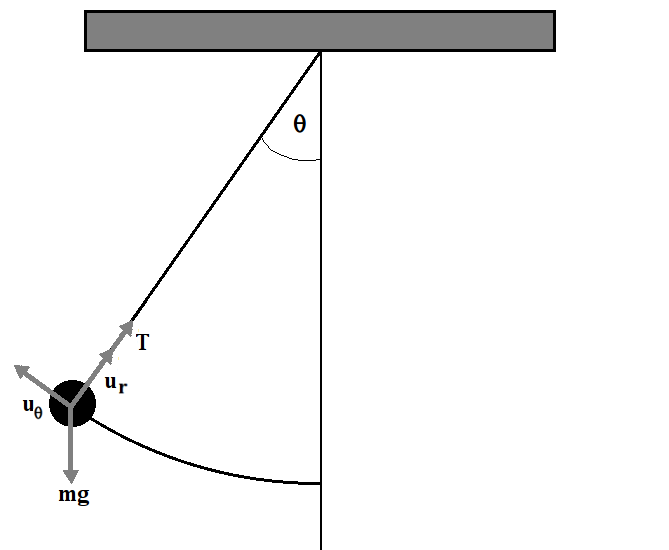
\includegraphics[width=0.50\textwidth]
	{./pictures/simple_pendulum.png}

	\caption{\small{Péndulo simple bajo la acción del campo gravitacional.}}
	
	\label{fig:simple_pendulum}
\end{figure}
%.........................................................................


En coordenadas polares se obtiene


%.........................................................................
%Movement equations
\begin{eqnarray}
\label{eq:simple_pendulum_1}
ml\dot \theta^2 &=& T - mg \cos \theta \\
\label{eq:simple_pendulum_2}
ml\ddot \theta &=& -mg \sin \theta
\end{eqnarray}
%.........................................................................


Como primera demostración computacional de este capítulo se solucionará el 
movimiento del péndulo simple a partir de las ecuaciones 
\ref{eq:simple_pendulum_1} y \ref{eq:simple_pendulum_2}. Para esto se 
asumirá que la amplitud de oscilación del péndulo es pequeña de tal forma 
que $\theta \approx \sin \theta$ y $\cos \theta \approx 1$, obteniendo


%.........................................................................
%Simplified equation
\eq{eq:simplified_pendulum}
{\ddot \theta = - \frac{g}{l} \theta}
%.........................................................................


Usando un ansatz de la forma $\theta(t) = e^{\lambda t}$ se llega a la
solución


%.........................................................................
%Approximate solution
\eq{eq:pendulum_solution}
{ \theta(t) = \theta_0 \sin ( \omega_0 t + \delta ) }
%.........................................................................
donde $\theta_0$ y $\delta$ son la amplitud y la fase respectivamente y 
constituyen las condiciones iniciales. La frecuencia $\omega_0$ está 
definida por 


%.........................................................................
%Frequancy
\eq{eq:freq_pedulum}
{ \omega_0 = \sqrt{ \frac{g}{l} } }
%.........................................................................

\

En el siguiente script de \python se grafica esta solución para diferentes
valores de la amplitud y la fase.

\newpage
%ccccccccccccccccccccccccccccccccccccccccccccccccccccccccccccccccccccccccc
%DEMO 2_01
\begin{listing}[style=python]
#!/usr/bin/env python
#==========================================================
# DEMOSTRACION 1
# Grafica de soluciones aproximadas del pendulo simple
#==========================================================
import numpy as np
import matplotlib.pylab as plt

def Theta(t):
    theta = theta0*np.sin( omega0*t + delta )
    return theta
    
#Gravedad
g = 9.8
#Longitud
l = 1
#Frecuencia
omega0 = np.sqrt( g/l )
#Tiempos
tiempo = np.arange( 0, 10, 0.1 )
    
#SOLUCION 1
#Amplitud
theta0 = 0.05
#Fase
delta = 0.0
#Grafica
plt.plot( tiempo, Theta(tiempo), label='solucion 1' )

#SOLUCION 2
#Amplitud
theta0 = 0.05
#Fase
delta = np.pi
#Grafica
plt.plot( tiempo, Theta(tiempo), label='solucion 2' )

#SOLUCION 3
#Amplitud
theta0 = 0.1
#Fase
delta = 0.0
#Grafica
plt.plot( tiempo, Theta(tiempo), label='solucion 3' )

plt.legend()
plt.show()
\end{listing}
%ccccccccccccccccccccccccccccccccccccccccccccccccccccccccccccccccccccccccc


El resultado que se obtiene es


%.........................................................................
%Simple Pendulum
\begin{figure}[htbp]
	\centering
	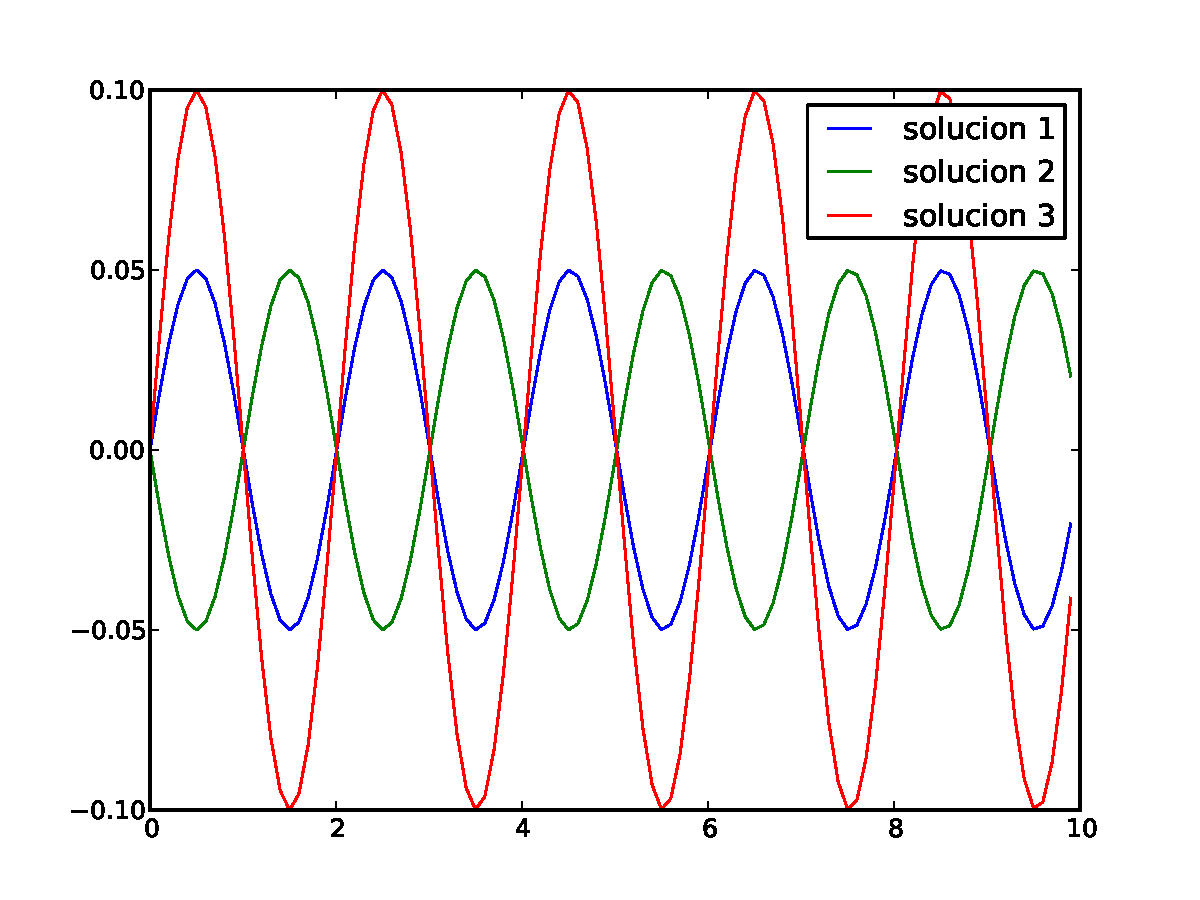
\includegraphics[width=0.8\textwidth]
	{./pictures/demo2_01.pdf}

	\caption{\small{Soluciones aproximadas obtenidas para el péndulo simple.}}
	
	\label{fig:approx_pedulum}
\end{figure}
%.........................................................................


En lo siguiente se explica cada porción de código.


%ccccccccccccccccccccccccccccccccccccccccccccccccccccccccccccccccccccccccc
%DEMO 2_01
\begin{listing}[style=python, numbers = none]
import numpy as np
import matplotlib.pylab as plt
\end{listing}
%ccccccccccccccccccccccccccccccccccccccccccccccccccccccccccccccccccccccccc
Esto corresponde al cargado de las librerías \numpy, bajo el alias de np y
\matplotlib bajo el alias de plt, ambas son necesarias para el desarrollo 
de todo el código.


%ccccccccccccccccccccccccccccccccccccccccccccccccccccccccccccccccccccccccc
%DEMO 2_01
\begin{listing}[style=python, numbers = none]
def Theta(t):
    theta = theta0*np.sin( omega0*t + delta )
    return theta
\end{listing}
%ccccccccccccccccccccccccccccccccccccccccccccccccccccccccccccccccccccccccc
En este parte se define la solución obtenida en la ecuación 
\ref{eq:pendulum_solution} para cualquier tiempo dado.


%ccccccccccccccccccccccccccccccccccccccccccccccccccccccccccccccccccccccccc
%DEMO 2_01
\begin{listing}[style=python, numbers = none]
#Gravedad
g = 9.8
#Longitud
l = 1
#Frecuencia
omega0 = np.sqrt( g/l )
#Tiempos
tiempo = np.arange( 0, 10, 0.1 )
\end{listing}
%ccccccccccccccccccccccccccccccccccccccccccccccccccccccccccccccccccccccccc
Se define la gravedad, la longitud de la cuerda (en metros), la frecuencia
de oscilación y finalmente, usando la función \texttt{arange} de la librería
\numpy, se cons\-truye un arreglo de tiempos donde es evaluada la solución, de 
0 a 10 segundos con saltos de 0.1.


%ccccccccccccccccccccccccccccccccccccccccccccccccccccccccccccccccccccccccc
%DEMO 2_01
\begin{listing}[style=python, numbers = none]
#SOLUCION 1
#Amplitud
theta0 = 0.05
#Fase
delta = 0.0
#Grafica
plt.plot( tiempo, Theta(tiempo), label='solucion 1' )
\end{listing}
%ccccccccccccccccccccccccccccccccccccccccccccccccccccccccccccccccccccccccc
La primera solución es obtenida para una amplitud de $\theta_0 = 0.05$ 
radianes y una fase $\delta = 0$. La última línea corresponde a la 
construcción de la gráfica de la solución. Para esto se usa la función 
\texttt{plot} de la librería \matplotlib. El primer argumento corresponde
a los datos asociados al eje x, en este caso \texttt{tiempo}, mientras el
segundo argumento son los datos asociados al eje y, en este caso la solución
evaluada en el tiempo, es decir \texttt{Theta(tiempo)}. El argumento 
\texttt{label} indica el nombre que tendrá la solución en la gráfica final,
esto se denomina etiqueta de la función.


%ccccccccccccccccccccccccccccccccccccccccccccccccccccccccccccccccccccccccc
%DEMO 2_01
\begin{listing}[style=python, numbers = none]
plt.legend()
plt.show()
\end{listing}
%ccccccccccccccccccccccccccccccccccccccccccccccccccccccccccccccccccccccccc
Finalmente se termina el script con la función \texttt{legend}, la cual 
muestra en pantalla las etiquetas puestas a cada gráfica. Y la función 
\texttt{show} que muestra en pantalla todas las soluciones.

\rule{14cm}{0.5mm}
%*************************************************************************


%*************************************************************************